\documentclass[10pt,twocolumn,letterpaper]{article}

\usepackage{cvpr}
\usepackage{times}
\usepackage{graphicx}
\usepackage{amsmath}
\usepackage{amssymb}
\usepackage{url}
\graphicspath{ {./images/} }

\usepackage[breaklinks=true,bookmarks=false]{hyperref}

\cvprfinalcopy

\begin{document}

%%%%%%%%% TITLE
\title{Artificial Intelligence and IOT based detection of COVID Hotspots}

\author{Akshat Goyal\\
International Institute of Information Technology\\
Professor CR Rao Rd, Gachibowli, Hyderabad, Telangana 500032\\
}

\maketitle

%%%%%%%%% ABSTRACT
\begin{abstract}
   The coronavirus pandemic has caused multiple issues for governments all over the world. The government is looking to lockdown the coronavirus hotspots. However, the hotspots are by virtue dynamic in nature and vary with the changing social interaction and needs of the people. Thus predicting regions of the probable hotspots is a challenging task. We propose an AI and IOT based novel solution to this problem which includes - a smart-thermometer which transmits its reading to the app~\cite{smart-thermometer}, an AI based smart doctor which helps you in identifying corona symptoms~\cite{smart-doctor} and informs govt. of the possible cases, and a Kalman Filter algorithm which uses this data to predict coronavirus hotspots~\cite{kalman-filter} and alerts nearby hospitals and health centers and govt.
\end{abstract}

%%%%%%%%% BODY TEXT
\section{Introduction}

The coronavirus pandemic has caused multiple issues for governments all over the world. From tracking cases to managing resources, the current situation has posed multiple challenges to the government. With the lockdown in place, our economy is suffering a huge blow. Instead of a complete lockdown in place,our government has resorted to placing lockdown only on the capable coronavirus hotspots. However The hotspots are by virtue dynamic in nature and vary with the changing social interaction and needs of the people. Thus predicting regions of the probable hotspots is a challenging task.


The rate of testing of coronavirus is not enough. Moreover visiting a doctor for Corona testing involves the risk of getting it even if you don’t have it in the first place. Therefore, we need an alternate online based solution which can do mass testing and inform the government of the possible hotspots and alert nearby hospitals and health centers about potential case spurts in their area, and notify them the quantity (based on the number of cases in the neighbourhood) of safety and medical equipment (such as ventilators, masks etc.) and medication to stack up.

%------------------------------------------------------------------------
\section{Literature Review}

There are numerous applications online that are working on the same idea.


A Kinsa company in the USA developed a smart thermometer to detect seasonal flu. A smart thermometer is a medical thermometer which is able to transmit its readings so that they can be collected, stored and analysed. They are now using it to detect coronavirus hotspots by detecting major clusters of fever-the most common symptoms of coronavirus. Smart thermometers are not available in India and many other countries.~\cite{smart-thermometer}


An app called - Babylon‘s uses AI technology to process various combinations of symptoms at a very high accuracy and speed. The system uses a chatbot to deal with - urgent but non-life-threatening conditions.~\cite{babylon}


Whereas, another app named - Pocket Doctor is a learning and educational app that only provides information regarding the Health & Medicine, human anatomy, body max index calculations and many more similar features. It also provided a health dictionary and based on which various symptoms can be analyzed.~\cite{doctor-pocket}


Similarly one of the most common medical apps is - BAIDU that uses an artificial intelligence with advanced deep learning and natural language processing technologies based chatbot system called Melody, to facilitate patients and doctors.~\cite{baidu-doctor}


However this BAIDU like chatbot apps are not available in India and these apps are not equipped to deal with coronavirus cases.

%------------------------------------------------------------------------
\section{System Architecture}

The project involves many key components,


1. Smart Thermometer -  Smart Thermometer uses IOT devices to transmit its readings to the app through wifi which is stored in the user's history and used by decision tree algorithm for smart doctor feature.~\cite{smart-thermometer}

\begin{center}
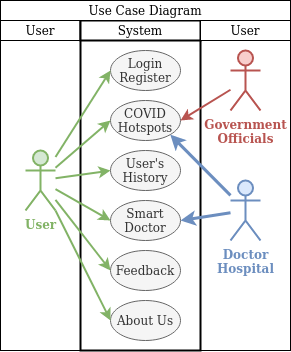
\includegraphics[width=1\linewidth]{uml_use_case_diagram.png}
\caption{Figure 2.1. UML Use Case Diagram}
\end{center}


2. Smart Doctor - The AI system uses a rational agent driven through a soft-bot with a goal based agent to diagnose and suggest health treatment. The precept given from the user input would be used to provide suggestions that are then searched from a knowledge base using a tree search algorithm.~\cite{smart-doctor}


The AI based smart doctor uses a decision tree algorithm which drives the perception based AI softbot questionnaire. We get new perception at every input from the user, which determines the next level of question, therefore the use of tree search algorithms facilitates the system through match strategies, if there is no match, and then the system would continue the loop until the end of the tree is reached.~\cite{smart-doctor}


User describes the symptoms through either voice or text. The voice is converted to text using google speech api and then text is processed using NLP, neural network techniques and then delivered to the decision tree.

\begin{center}
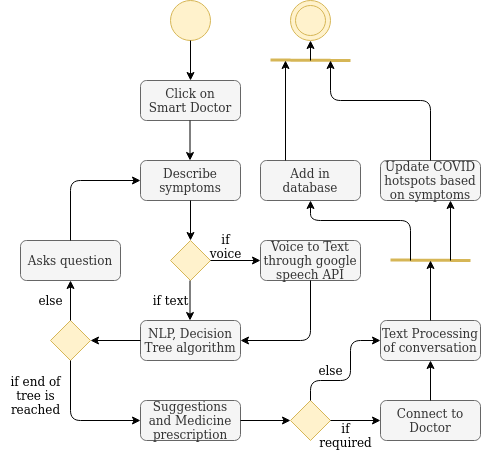
\includegraphics[width=1\linewidth]{uml_state_diagram.png}
\caption{Figure 2.2. UML State Diagram Of Smart Doctor}
\end{center}


3. Hotspots - This is the major component of the project. This feature shows the COVID hotspots areas in the map. based on the data collected through smart thermometer and smart doctor.~\cite{smart-thermometer}


Moreover, it uses Kalman filter algorithm, a fitting time series analysis and statistical algorithms to produce the best short term prediction. An adaptive online Kalman filter provides us a very good one-day ahead prediction for each region. It uses the total  confirmed, death, recovered, suspected COVID cases collected from smart thermometers, smart doctor data and from government officials and generates a day ahead prediction for each case.~\cite{kalman-filter}


It alerts the nearby hospitals and health centers about potential case spurts in their area, and notify them the quantity (based on the number of cases in the neighbourhood) of safety and medical equipment (such as ventilators, masks etc.) and medication to stack up and informs the government to start testing the area and impose lockdown if necessary.

\begin{center}
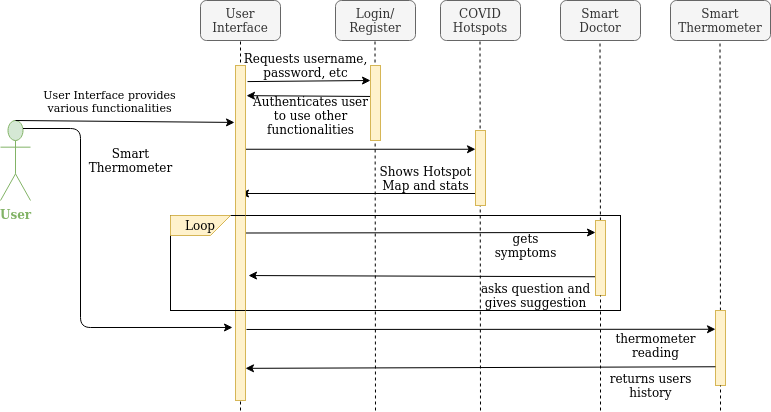
\includegraphics[width=1\linewidth]{images/uml_sequence_diagram.png}
\caption{Figure 2.3. UML Use Sequence Diagram}
\end{center}

%------------------------------------------------------------------------
\section{Conclusion and Future Work}

Artificial Intelligence is becoming a norm of every technology development. The project uses an AI system to develop an efficient chatbot system based on rational agent with tree searching algorithm and knowledge base of medical data. The data collected from smart doctor and smart thermometer is used to decide the probability of an area to be a COVID hotspot. The project then uses the Kalman Filter algorithm to do the one-day ahead prediction for each case - confirmed, death, recovered, for each region.


In the future, the system needs to increase its database to improve its diagnostics. Also we can add a Contact Tracing feature in the app which will help in tracing the contacts of the suspects and help in better predicting the hotspots. Apple and Google are working on it and will be providing an api from May for contact tracing. We can use that api in our app.~\cite{contact-tracing}


{\small
\bibliographystyle{ieee}
\bibliography{references}
}

\end{document}
